\documentclass[tikz,border=6pt]{standalone}
\usepackage{amsmath,amssymb}
\usetikzlibrary{calc}
\begin{document}
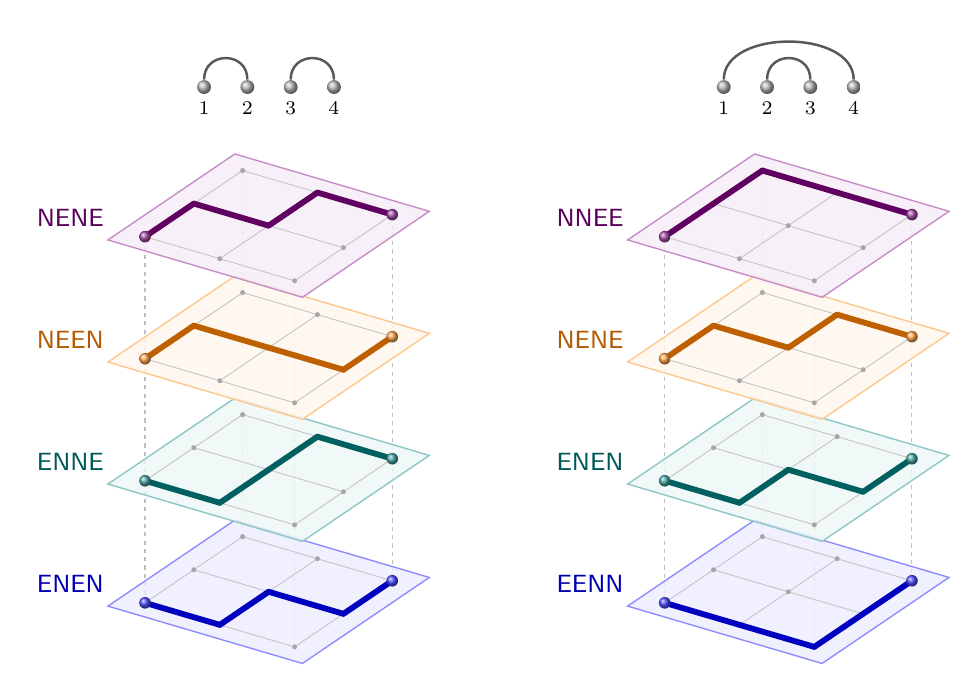
\begin{tikzpicture}[
  x={(0.95cm,-0.28cm)}, y={(0.62cm,0.42cm)}, z={(0cm,1cm)},
  plane/.style={fill=#1!7,draw=#1!45,line width=0.5pt,fill opacity=0.82},
  gridl/.style={draw=black!22,line width=0.35pt},
  pathl/.style={draw=#1!75!black,line width=2.1pt,line cap=round,line join=round},
  vert/.style={circle,shading=ball,ball color=#1!70,inner sep=0pt,minimum size=4.2pt},
  post/.style={draw=black!25,line width=0.4pt,dash pattern=on 1.5pt off 1.5pt},
  word/.style={font=\small\sffamily,anchor=east}]

% one layer: #1 shift in x (screen), #2 height, #3 colour, #4 list of steps (0 = E, 1 = N), #5 label
\newcommand{\layer}[5]{%
  \begin{scope}[xshift=#1cm]
    \filldraw[plane=#3] (-0.3,-0.3,#2) -- (2.3,-0.3,#2) -- (2.3,2.3,#2) -- (-0.3,2.3,#2) -- cycle;
    \foreach \u in {0,1,2} {\draw[gridl] (\u,0,#2) -- (\u,2,#2); \draw[gridl] (0,\u,#2) -- (2,\u,#2);}
    \foreach \u in {0,1,2} \foreach \v in {0,1,2} \fill[black!35] (\u,\v,#2) circle (0.9pt);
    \coordinate (P) at (0,0,#2);
    \def\px{0}\def\py{0}
    \foreach \s [count=\i] in {#4} {
      \ifnum\s=0 \pgfmathtruncatemacro{\nx}{\px+1}\pgfmathtruncatemacro{\ny}{\py}
      \else \pgfmathtruncatemacro{\nx}{\px}\pgfmathtruncatemacro{\ny}{\py+1}\fi
      \draw[pathl=#3] (\px,\py,#2) -- (\nx,\ny,#2);
      \global\let\px\nx \global\let\py\ny
    }
    \node[vert=#3] at (0,0,#2) {};
    \node[vert=#3] at (2,2,#2) {};
    \node[word,text=#3!70!black] at (-0.55,0.2,#2) {#5};
  \end{scope}}

% left family: M = {{1,2},{3,4}}
\foreach \h in {0,1,2} \foreach \u in {0,2} \foreach \v in {0,2}
  \draw[post] (\u,\v,1.55*\h) -- (\u,\v,1.55*\h+1.55);
\layer{0}{0}{blue}{0,1,0,1}{ENEN}
\layer{0}{1.55}{teal}{0,1,1,0}{ENNE}
\layer{0}{3.1}{orange}{1,0,0,1}{NEEN}
\layer{0}{4.65}{violet}{1,0,1,0}{NENE}

% right family: M = {{1,4},{2,3}}
\begin{scope}[xshift=6.6cm]
\foreach \h in {0,1,2} \foreach \u in {0,2} \foreach \v in {0,2}
  \draw[post] (\u,\v,1.55*\h) -- (\u,\v,1.55*\h+1.55);
\end{scope}
\layer{6.6}{0}{blue}{0,0,1,1}{EENN}
\layer{6.6}{1.55}{teal}{0,1,0,1}{ENEN}
\layer{6.6}{3.1}{orange}{1,0,1,0}{NENE}
\layer{6.6}{4.65}{violet}{1,1,0,0}{NNEE}

% the matchings above the columns (screen coordinates)
\newcommand{\matchrow}[2]{%
  \begin{scope}[x=1cm,y=1cm,xshift=#1cm,yshift=6.55cm]
    \foreach \i in {1,2,3,4} \node[circle,shading=ball,ball color=gray!55,inner sep=0pt,minimum size=5pt] (m\i) at (0.55*\i,0) {};
    \foreach \i in {1,2,3,4} \node[font=\scriptsize,below=2pt] at (m\i) {\i};
    #2
  \end{scope}}
\matchrow{0.2}{\draw[line width=0.9pt,black!65] (m1) to[out=90,in=90,looseness=1.7] (m2);
               \draw[line width=0.9pt,black!65] (m3) to[out=90,in=90,looseness=1.7] (m4);}
\matchrow{6.8}{\draw[line width=0.9pt,black!65] (m1) to[out=90,in=90,looseness=1.0] (m4);
               \draw[line width=0.9pt,black!65] (m2) to[out=90,in=90,looseness=1.7] (m3);}
\end{tikzpicture}
\end{document}
